\chapter{Surface Codes} 
\label{ch:SurfaceCodes}

\section{Motivation}

The toric code is the simplest and most elegant of the class of topological codes \cite{topological_codes}. The code uses $2n^2$ physical qubits to encode two logical qubits. The code's properties are usually studied in the large-$n$ limit, where it has been shown that the ideal code can protect against errors on $18.9\%$ of the phsyical qubits \cite{bombin12}. In practice the threshold obtained depends not only on the code, but also on the decoding algorithm used. The search for an efficient, high-threshold decoding alogithm has attracted a lot of attention recently, and there are a number of decoders that approach the theoretical threshold \cite{wooton_mcmc1, poulin_renormalisation, poulin_renormalisation2} [TODO need a reference for best threshold using Edmonds type approach].

When the operations required to perform the code are taken into account, the error rates tolerated fall to $0.75\% - 1.4\%$ depending on the error model \cite{raussendorf07, fowler11, ghosh_fowler}, which seems less impressive when compared with tolerated error rates of $3.2\%$ \cite{?Knill} demonstrated for concatenated codes. The advantage of the toric and other stabiliser codes is that only local operations are required, making a scalable physical implementation more realistic.

In this paper we look towards an experimental realisation of the toric code and study the code for small values of $n$. We pre-compute a decoding library, an approach that quickly becomes intractible for values of $n$ above those considered here, but has the advantage that we obtain a provably optimum decoding success rate. We use our pre-computed decoder to assess the \textit{encoding power} of the code: we say the code has positive encoding power if the encoded qubits exhibit a lower error rate than the same number of unencoded qubits subjected to the same noise.

\section{Review of the Toric Code}

The toric $2n$-code (Fig. \ref{4-code}) uses $2n^2$ physical qubits to encode $2$ logical qubits. The \textit{codespace}, the subspace  that the code states inhabit, is most elegantly described using the \textit{stabiliser formalism} - by specifying a set of commuting operators with respect to which the state is invariant. For example, the Bell singlet state $\vert01\rangle - \vert10\rangle$ is given in stabiliser formalism by $\{ -X_1 X_2, -Z_1 Z_2 \}$ (the symmetry of which makes it clear that the state has the same form when written in the $X$ basis). By specifying $n$ independent, commuting, binary-outcome stabilisers we fully define an $n$ qubit state.

To describe the code, it is useful to picture the $2n^2$ physical qubits positioned on the odd diagonals of a $2n \times 2n$ lattice (i.e. in the positions with coordinates $(i,j)$, where $i+j$ is odd). The remaining positions will represent the stabilisers used to define the code. The stabilisers fall into two distinct families: the $X-$stabilisers, pictured on the even rows (those sites with coordinates $(i,j)$ where $i$ and $j$ are both even); and the $Z-$stabilisers, pictured on the odd rows. The $X/Z$-stabiliser at a given site represents the product of the four $X/Z$ operations on the neighbouring physical qubits (see Fig. \ref{4-code}). The `toric' nature of the code comes from identifying opposite edges of the lattices in what we consider to be neighbouring physical qubits. 

\begin{figure}[htb]
  \begin{center}
    \includegraphics[width=5cm]{assets/4-code.pdf}
  \end{center}
  \caption{Qubit lattice for the $4$-code. $s_i^X$ and $s_i^Z$ are $X$- and $Z$-stabilisers represented by the sites respectively. $q_i$ are qubits. By way of example, $s_0^X = X_0 X_2 X_1 X_6$ and $s_0^Z = Z_3 Z_4 Z_2 Z_0$.}
  \label{4-code}
\end{figure}

As all the stabilisers commute with one another, a given set of stabiliser measurement outcomes, or {\it syndrome}, can be used to define the codespace. If the outcome of the measurement is a $-1$ we say that the stabiliser has fired. Only $n^2-1$ of the $X$-stabilisers and $n^2-1$ of the $Z$-stabilisers are actually independent: the final stabiliser is the product of the others, so the outcome of the final stabiliser measurement is determined by the previous outcomes. This places the restriction on the set of possible syndromes, $A$, that the total number of firing stabiliser sites must be even and means that the codespace is the size of two qubits.

To fully define the state we must add another two independent, commuting operators to the set. We define $X_h$ (horizontal X) to be the product of $X_i$s acting on qubits in an even row, $X_v$ (vertical X) the product of $X_i$s acting on qubits in an even column, and similarly, $Z_h$ to be $Z_i$s on an odd row, and $Z_v$ to be $Z_i$s on an odd column. Any of the pairs $\{X_v, X_h\}$, $\{X_v, Z_v\}$, $\{Z_v, Z_h\}$, and $\{Z_h, X_h\}$ will suffice to fully define the state. The remaining pairs, $\{X_v, Z_h\}$ and $\{X_h, Z_v\}$, satisfy the standard qubit commutation relation, $[X, Z] = 2iY$, and so we can use this set of \textit{logical operators}, $L = \{X_v, X_h, Z_v , Z_h\}$, to define a pair of independent \textit{logical qubits}. 

Now that we have defined the codespace and given a basis for our logical qubits, we move on to looking at error correction. For the rest of the paper we work in the codespace given by the \textit{zero-syndrome}, where each stabiliser outcome is $+1$ (where no stabiliser sites fire). The first stage of the error correction step is to measure all the stabilisers. If any of the stabiliser sites fire, we know that we are no-longer in the codespace and must take steps to rectify the situation.

\begin{figure}[htb]
  \begin{center}
    \includegraphics[width=8cm]{assets/4-code_error_correct.pdf}
  \end{center}
  \caption{Two different possible matchings for an $X$-flip error on $q_4$. The correction on the left introduces a logical error, while the one on the right does not.}
  \label{4-code_error_correct}
\end{figure}

Any error on a single physical qubit can be considered a mixture of $X$, $Z$ and $Y = XZ$ errors, up to global phase. It therefore suffices to be able to correct these types of errors. An $X$ error on a single qubit will cause both neighbouring $Z$-stabiliser sites to fire, but will be undetected by the $X$-stabilisers. Similarly, $Z$ errors will be detected by the $X$-stabiliser measurements and $Y$ errors by both sets of stabiliser measurements. If qubit errors do not occur in isolation, stabiliser sites fire at either end of the string of errors. To move back into the codespace we must apply operations to the physical qubits to prevent these stabilisers from firing: we must apply strings of operations each of whose ends connect two firing stabiliser sites. We call such a set of operations a \textit{matching} for the syndrome.

While such a matching is guaranteed to return us to the codespace, it is possible that it will also alter the state of the logical qubits. It is useful to consider the error introduction, $e$, and error correction, $m$, as jointly perfoming an operation $r=em$. As $r$ maps the codespace to itself, it can be written as a product of stabilisers and logical qubit operators. If $r$ is a product of stabilisers only then the logical qubit state remains unaltered. Geometrically this corresponds to $r$ being represented as product of operators forming trivial loops or loops that wrap the torus an even number of times in each direction. 

A \textit{decoder} takes a given sydrome, $a$, and returns a matching $m$. The aim of the decoding step is to return to the codespace without altering the logical qubit state. Unfortunately, given a syndrome, $a$, it is impossible to determine the underlying errors that occurred, only that they must belong to a set $E_a$ of errors consistent with the syndrome. Moreover the logical error introduced by the operation $r = em$ is not the same for all $e \in E_a$ regardless of the choice of $m$. It is thus impossible to have a perfect decoder, and we must be content with a decoder offering a reasonable success probability in a reasonable amount of time.

It is worth noting that it is not necessary to physically perform the matching operation on the physical qubits; as a Pauli operation on a given qubit can just be considered a redefinition of the local basis, it is enough to keep track of the operations that would be performed at each stage, provided these are taken into account on any further operations that are performed.

\section{error models}

We consider deploarising noise of the form
\begin{equation} \label{noise_eq}
  \begin{split}
  D(\rho) = p_x X\rho X + & p_z Z\rho Z + p_y Y\rho Y \\
  & + (1- p_x - p_y - p_z)\rho
  \end{split}
\end{equation}
in two different cases:
\begin{enumerate}
  \item Single channel noise: $p_y = p$, $p_x = p_z = 0$
  \item Full channel noise: $p_x = p_y = p_z = p/3$
\end{enumerate}

We also consider the effect of stabiliser sites mis-reporting the stabiliser measurement outcomes: that with some probability, $q$, the stabiliser reports that it fired (/did not fire) when it did not (/did). The normal approach here is to consider multiple faulty stabiliser evaluations as extending the code into a third dimension. By observing the stabiliser outcomes over multiple rounds it is possible to increase the chance of correctly identifying any mis-reported outcomes.

We just consider a single round of stabiliser evaluation, and so this extra information is not available to us. Instead we try to identify and correct the right syndrome based on the sydrome we see. Even in multi-round systems the final step will look like this and so our results are an upper bound on the possible decoding probabilities for small systems.

\section{Experimental suggestion}

Our aim in this section is to provide a criterion which an experimentalist can use to verify whether a given candidate toric code set-up is providing protection.

Our criterion is based on the observation that the $2$-code is essentially equivalent to two unprotected qubits: the sydrome outcome is always $+1$ so we are unable to even detect errors and the logical operations reduce to single qubit operations. By comparing the performance of the candidate code system against that of the $2$-code we are able to say whether the candidate system is exhibiting protective power. 

We do not specify the decoder that the experimentalist must use for the larger code (decoding is trivial in the $2$-code), but in the remainder of the paper develop a provably-optimal decoder for small systems under the given error channels and use this to estimate the values of $p$ and $q$ that the experimentalist needs to obtain to satisfy the criterion. In the analysis that follows in the paper we assume that the stabiliser mis-reporting and physical qubit errors are independent events. A round of stabilisers is permitted to introduce physical qubit errors, but these must be sprinkled evenly over the lattice and not be correlated with mis-reporting sites. If strong correlations were to exist a modified decoder would give a better chance of satisfying the criterion.

We assume that an experimentalist has the ability to perform all $X$- and $Z$-stabiliser measurement operations and the logical X measurements. In a large code the logical operations are potentially tricky, given their non-local nature. Here, due to the size of the codes considered, the logical operations actually involve fewer qubits than the stabilisers, and so are likely to be less technically demanding.

Our experimental proposal is as follows:
\begin{enumerate}
  \item Measure  $X_v$, $X_h$, and the stabilisers to find intitial syndrome $a'_i$ and logical qubit states $(x^v_i, x^h_i)$\label{first_step}
  \item Wait. Manually introduce noise if required.
  \item Measure $X_v$, $X_h$, and the stabilisers to find final syndrome $a'_f$ and logical qubit states $(x^v_f, x^h_f)$
  \item Decode the calculated syndrome, $a' = a'_i \text{\,XOR\,} a'_f$, to find matching $m$ \label{decode_step}
  \item Modify $(x^v_f, x^h_f)$ to reflect what the outcomes would have been if we had applied $m$ before measurement to find $(x^v_m, x^h_m)$
  \item If $(x^v_i, x^h_i) = (x^v_m, x^h_m)$ count the round as a success; if not, count the round as a failure.\label{last_step}
  \item Repeat steps \ref{first_step} to \ref{last_step} many times to calculate an experimental successful decoding probability $P_\text{d}^\text{expt}$
\end{enumerate}

We then repeat this procedure for the $2$-code and compare the results: if the larger system outperforms the $2$-code protection is provided. 

In the rest of the paper we assume that we start in a known initial state, corresponding to the zero-syndrome and known logical states. In the experimental procedure described above this is not the case, as our initial stabilisers may have mis-reported. Thankfully in the decoding step (\ref{decode_step}) we are concerned only with the difference between the initial and final sydromes, and so the two situations are equivalent albeit with a modified mis-reporting probability $q$. In order to interpret the results given later we must set $q = 2q_\text{expt}(1-q_\text{expt})$, where $q_\text{expt}$ is the actual stabiliser measurement mis-reporting probability for the system. An improved experimental procedure would involve aborting any experiment where an odd number of stabilisers fire in the initial measurement, which would make initialisation mis-reports an $O(q_\text{expt}^2)$ event and allow $q \approx q_\text{expt}$ for small $q_\text{expt}$.

\section{decoders}

When discussing decoders it is useful to start with an arbitrary matching, $m^*(a)$, for the given syndrome $a$. This matching allows us to split the possible physical qubit error configurations $e \in E_a$ into subsets $E_{a,l}$ based on the corresponding logical operation, $l\in L$, that is performed by the overall operation $r = em^*$.

We first consider the probability that we see sydrome $a$ and decode it with $m^*(a)$ we introduce the logical operation $l$ on the encoded qubits,
\begin{align}
  p(l \vert a) = \sum_{e \in E_{a,l}} \frac{p(e)}{p(a)}. 
\end{align}
For each stabiliser outcome $a$ we identify the most likely logical error $l_a$, such that $p(l_a \vert a)$ obtains a maximum. In cases where the most likely logical error is not unique we pick arbitrarily between the candidates. The overall successful decoding probability is 
\begin{align}
  P_d &= \sum_{a \in A} p(l_a \vert a)p(a) \\
  &= \sum_{a \in A} \max_{l\in L} \left\{ \sum_{e \in E_a} \frac{p(e)}{p(a)} \right\} p(a) \\
  &= \sum_{a \in A} \max_{l\in L} \left\{ \sum_{e \in E_a} p(e) \right\} \label{truthful_prob}
\end{align}

When considering mis-reported stabiliser outcomes we must relax the restriction that there will be an even number of firing stabiliser sites. We let $A'$ be the set of all possible stabiliser outcomes $A' = \{0, 1\}^{\otimes n^2}$. If we are to successfully decode a syndrome $a'$, we must first identify the correct sydrome $a$, on which to perform the arbitrary matching, and then identify the most likely logical error $l_a$ to correct. If we identify the wrong $a$ the final state will not even be in the code space. Given $a'$ we must pick $a$ and $l$ to provide the maximum probability of a successful decoding in the case of mis-reporting stabiliser outcomes:
\begin{align}
  P'_d &= \sum_{a' \in A'} p(\text{success} \vert a') p(a') \\
  &= \sum_{a'\in A'} \max_{a \in A} \left\{ p(l_a \vert a) p(a \vert a') \right\} p(a')\\
  &= \sum_{a'\in A'} \max_{a \in A} \left\{ \max_{l \in L} \left\{\sum_{e \in E_a} \frac{p(e)}{p(a)} \right\} p(a \cap a') \right\}\\
  &= \sum_{a'\in A'} \max_{a \in A} \left\{ \max_{l \in L} \left\{\sum_{e \in E_a} p(e) \right\} p(a' \vert a) \right\} \label{lying_prob}
\end{align}

\section{Precomputed decoder}

While equations (\ref{truthful_prob}) and (\ref{lying_prob}) are conceptually simple, calculations are beset by difficulties due to the rapid growth in the size of the sets $E_{a,l}$, $A$, and $A'$: in the single noise channel case for the $2n$-code $|E_{a,l}| = |A| = 2^{n^2-1}$; for the full noise channel $2n$-code $|E_{a,l}| = |A| = 2^{2n^2 - 2}$. For example, the total number of error configurations, $|E|$, for the $6$-code is $2^{36}$, which would require $\sim200$GB of storage space.

Thankfully, it we do not need the complete set of error configurations to compute the value of $p_\text{success}$ in eq (\ref{truthful_prob}). For each configuration $e\in E$ the probability is
\begin{align}
  p(e) = (1-p)^{2n^2 - n(e)} p^{n(e)}
\end{align}
where $n(e)$ counts the number of errors in error configuration $e \in E$. When summing over the errors consistent with a given logical error and syndrome we get
\begin{align}
  \sum_{e \in E_{a,l}} p(e) &= \sum_{e \in E_{a,l}} (1-p)^{2n^2 - n(e)} p^{n(e)} \\
  &= (1-p)^{n^2} \sum_{i = 0}^{2n^2} d_{a,l}^{(i)} \left(\frac{p}{1-p}\right)^i \\
  &=: (1-p)^{n^2} \chi_{a,l}\left(\frac{p}{1-p}\right)
\end{align}
where $d_{a,l}^{(i)} = \vert \left\{e \in E_{a,l} : n(e)=i \right\} \vert$ and we have used the final line to define the characteristic function $\chi_{a,l}$ of the class $E_{a,l}$. By computing and storing the coefficients $d_{a,l}$ we are able to calculate the success probabilities for a range of values of $p$.

The full source code used for our calculations, along with the computed tables of characteristic function coeffients, is available online \cite{?}.

\section{Single channel noise}

We first envisage a system where there is a single dominant error channel. Without loss of generality we take this to be the $Y$ channel, setting $p_y = p$ and $p_x = p_z = 0$ in equation (\ref{noise_eq}). In this choice we optimize the code against the given dominant error: $Y$ errors are detected in both the $X$ and $Z$ syndromes, giving us the most information to work with during the decoding step.

\begin{figure}[htb]
  \begin{center}
    \includegraphics[width=8cm]{assets/y_truthful.pdf}
  \end{center}
  \caption{Success probabilities for toric code on a grid that suffers only from y errors. We use x- and  z-stabiliser information to correct y-errors, in order to recover the x or z components of the encoded qubits.}
  \label{y_truthful}
\end{figure}

We find that the first non-trivial code, the $4$-code, offers encoding power in this scenario (Fig. \ref{y_truthful}). The $4$-code has both error-detect and error-correct capability and outperforms the $2$-code up to a physical qubit error probability of around $20\%$. It is worth contrasting this with the $4$-code protecting against single channel $X$ noise, which offers no error-correct capabilities: even a single isolated error has a decoding probability of at most $0.5$, as there are always two equally likely matchings (see Fig. \ref{4-code_error_correct}).

\begin{figure}[htb]
  \begin{center}
    \includegraphics[width=8cm]{assets/y_lying.pdf}
  \end{center}
  \caption{Decoding success probabilities for the full quantum $6$-code with mis-reported stabiliser outcomes.}
  \label{y_lying}
\end{figure}

When protecting against single channel $Y$ noise, the $4$-code shows remarkable resilience against stabiliser outcome mis-reports, being able to comfortably deal with mis-reporting probabilities in the region of $5\%$ (Fig. \ref{y_lying}).

\section{Full channel noise}

We now look at the full depolarizing noise model, taking $p_x = p_y = p_z$ in equation (\ref{noise_eq}). 

\begin{figure}[htb]
  \begin{center}
    \includegraphics[width=8cm]{assets/full_truthful.pdf}
  \end{center}
  \caption{Success probabilities for full toric code with perfect stabiliser outcome reporting.}
  \label{full_truthful}
\end{figure}
\begin{figure}[htb]
  \begin{center}
    \includegraphics[width=8cm]{assets/full_lying.pdf}
  \end{center}
  \caption{Decoding success probabilities for the full quantum $6$-code with stabilser outcome mis-reporting.}
  \label{full_lying}
\end{figure}


In this case the $4$-code does not offer any encoding power over the $2$-code. The $4$-code has error-detect capacity but limited error-correct capacity, exemplified in its ability to correct isolated $X$ or $Z$ errors with probability about $0.5$. The $6$-code is the first code to offer encoding power (Fig. \ref{full_truthful}), outperforming the $2$-code for $p \le \sim 0.15$.

We looked at mis-reported stabiliser outcomes for the $6$-code (Fig. \ref{full_lying}). Due to computational constraints we were only able to find a lower bound for $p_{\text{success}}(6, p, q)$. This was obtained by modifying equation (\ref{lying_prob}) to maximise only over $a$ close to $a'$:
\begin{align} \label{approx_eq}
  P'_d= \sum_{a'\in A'} \max_{a \in N(a',x)} \left\{ \max_{l \in L} \left\{\sum_{e \in E_{a,l}} p(e) \right\} p(a' \vert a) \right\}
\end{align}
where $N(a', x) = \left\{a \in A : d(a', a) \leq x \right\}$ with $d(a', a)$ the number of stabilisers where $a'$ differs from $a$. We took $x = 2$ to produce a rough region, and then used $x=4$ to refine the boundary. The $6$-code is able to tolerate far lower stabiliser outcome mis-reporting rates, in the region of $0.5 - 1\%$.

\section{Conclusion}

We have provided a protocol and pre-computed decoder for demostrating toric encoding size at minimal scale. The $2n$-code requires a minimum of $2n^2$ physical code qubits, plus an auxiliary qubit with which we must be able to perform CNOT operations with any of the code qubits. For the $4$-code this is a requirement of $9$ qubits and for the $6$-code the requirement is $19$ qubits. The error rates provided are not unrealistic for current experimental systems. 

